\documentclass[a4paper]{paper}
\usepackage[utf8]{inputenc}
\usepackage{xcolor}
\usepackage{graphicx} 

\begin{document}
\title{A second look at the health of the Go ecosystem}
\author{Ingvar Mattsson}

\maketitle

\section{Background}

The root inspiration for this investigation and report was trying to
use Athens, with a validating web-hook, for a company concerned with
what is brought in from external sources.

In the initial setup, there were three intentional (and one
non-intentional) way a package could fail validation. It could have
file(s) that triggered a vulnerability scanner, it could fail to
build, it could have failing unit tests. Or, unintended, either {\tt go
mod download} or {\tt go list -json}\footnote{One possible reason for this is that the GitHub repo has been moved, causing a skew between the downloaded URL and that in the go.mod file} could fail.

It soon became evident that ``has failing unit tests'' was not a
feasible\footnote{Part of this is that over time, multiple ``go vet''
  errors have been promoted test errors} criterion. It eventually
became evident that ``has failing build targets'' was also not
feasible.

This raised a question in the author's mind. What is the current state
of health of the Go eco-system? A previous investigation answered some of these questions, but it left sufficient scope for more questions to be asked (and refining the previous answers).

\section{Methodology}

In order to investigate what the current state of health of the Go
eco-system, you need to compile a lot of Go packages. You also need to
do some statistics on them.

In order to more easily get multiple modules, at various versions,
compiled through an instrumented build environment, the author built
an environment consisting of a validator (custom Go code), Athens
(pre-existing Docker container), and an instrumented build environment
(custom Python, in a Docker container).

\begin{figure}[ht]
  \label{fig:architecture}
  \caption{Rough system architecture, depicting JSON requests, module requests and execution with different arrows}
  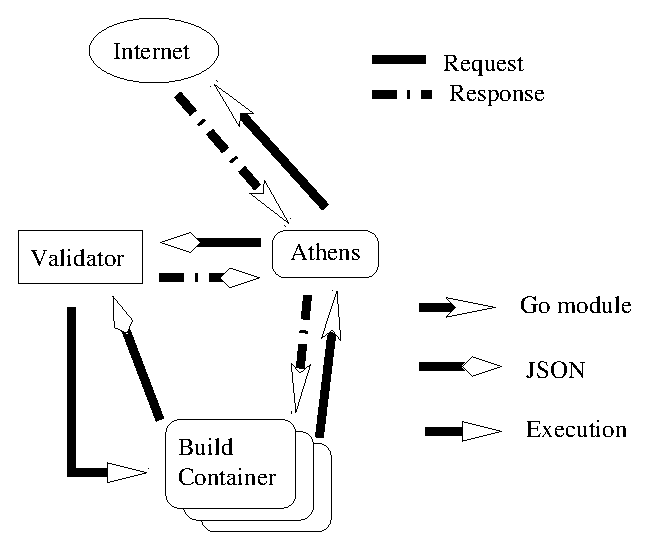
\includegraphics{architecture.eps}
\end{figure}


The validator considers all module/version tuples as valid. If the
specific module/version tuple has not been seen before, a build of
that is started\footnote{Technically, placed in a build queue}. The
validator limits builds to at most five concurrent ones, this is to
preserve some responsitivity on the test machine. It is possible to
increase the build parallelism by having more ``build workers''. The
number of build workers is set at compile time.

The custom build environment then reports back some general statistics
(did ``go mod download'' work, could we list all targets in the
downloaded code, did all builds succeed, did all tests succeed, how
many build/test targets, did go vet pass\footnote{This is a new test
  for this report}, and (on failure) what build/test targets
failed). The build environment is set up to use the Athens instance as
its GOPROXY, making it much easier to get a wide spectrum of code
scanned, as all transitive dependencies from the seed modules end up
being processed.

The validator periodically writes its current data set to disk. There
is also a web endpoint that triggers a save when accessed. The
validator will only create a new save file if there's been any
changes\footnote{Note, a ``change'' really means ``there has been
  build results reported'', in practice this is enough in the early
  stages of data gathering.}  since the last save.

To seed the scan, a few packages were manually started within the
build container, using the same environment as that set up by the
validator. For more details, see the section on seed packages.

The source code for the tabulator, the validation web-hook framework
and the build instrumentation can be found at
https://github.com/vatine/gochecker/ .

\section{The numbers}

Here are some numbers distilled from the investigation. For the
breakdown on failing build/test cases, the mean has only been done for
module/versions with at least one failure. The number of packages with
download problems is over-reported, as it includes: packages with a
name that differs from the requested in their go.mod, packages with a
version number that doesn't parse, and packages that simply do not
exist at this point in time.

\begin{table}[ht]
\caption{Build target statistics}
\label{table:build}
\begin{tabular}{|l|r|}
 \hline
  Packages processed & 4326 \\
  Packages failed to download & 1535 \\
  No build failures & 2604 (60.194175\%) \\
  No vet failures & 1789 (41.354600\%) \\
  No fmt failures & 4326 (100.000000\%) \\
  No test targets & 748 (17.290800\%) \\
 \hline
  Mean build targets (all modules)& 32.659270 \\
  stddev & 153.801803 \\
  Median build targets & 2 \\
  75th percentile \# of build targets & 10 \\
  90th percentile \# of build targets & 49 \\
  95th percentile \# of build targets & 185 \\
  99th percentile \# of build targets & 412 \\
  Max \# of build targets & 2674 \\
 \hline
  Mean build targets (at least one buildable)& 35.276904 \\
  stddev & 159.558912 \\
 \hline
  Mean failed build targets (all modules)& 20.178687 \\
  stddev & 147.212632 \\
 \hline
  Mean failed build targets (at least one failed)& 58.040559 \\
  stddev & 245.280695 \\
 \hline
  Mean failed vet targets (all modules)& 22.294267 \\
  stddev & 147.749693 \\
 \hline
  Mean failed vet targets (at least one failed)& 43.522112 \\
  stddev & 204.207778 \\
 \hline
\end{tabular}
\end{table}

\begin{table}[ht]
\caption{Test target statistics}
\label{table:test}
\begin{tabular}{|l|r|}
 \hline
  Packages seen & 4326 \\
  No test failures & 2165 (50.046232\%) \\
  No test failures (with tests) & 1417 (39.603130\%) \\
  No build failures, but test failures & 670 (15.487748\%) \\
  No tests & 748 (17.290800\%) \\
 \hline
  Mean failed test targets for passed builds (all) & 1.356716 \\
  stddev & 1.128344 \\
 \hline
  Mean failed test targets for passed builds (at least one fail) & 1.356716 \\
  stddev & 1.128344 \\
 \hline
  Mean failed test targets, all packages& 7.093012 \\
  stddev & 14.636305 \\
 \hline
  Mean failed test targets, packages with at least one test failure& 7.888832 \\
  stddev & 15.231140 \\
 \hline
\end{tabular}
\end{table}

\begin{table}[ht]
\caption{Most versions per module that  download}
\label{table:versions}
\begin{tabular}{|l|r|}
\hline
 golang.org/x/sys & 169 \\
 golang.org/x/tools & 139 \\
 google.golang.org/genproto & 130 \\
 golang.org/x/net & 109 \\
 google.golang.org/api & 62 \\
 cloud.google.com/go & 47 \\
 golang.org/x/crypto & 42 \\
 github.com/Azure/go-autorest/autorest & 31 \\
 google.golang.org/grpc & 28 \\
 github.com/prometheus/common & 27 \\
\hline
\end{tabular}
\end{table}
\begin{table}[ht]
\caption{Most versions per module that fail to download}
\label{table:failversions}
\begin{tabular}{|l|r|}
\hline
 github.com/hashicorp/consul & 72 \\
 golang.org/x/tools & 54 \\
 github.com/Azure/go-autorest & 53 \\
 google.golang.org/grpc & 40 \\
 github.com/hashicorp/vault & 37 \\
 contrib.go.opencensus.io/exporter & 36 \\
 golang.org/x/crypto & 34 \\
 github.com/aws/aws-sdk-go & 33 \\
 golang.org/x/exp & 21 \\
 github.com/Azure/go-autorest/autorest & 21 \\
\hline
\end{tabular}
\end{table}


\subsection{Download problems}

All in all, only 340 out of 5108 packages\footnote{Strictly speaking
  module/version pairs} had a problem, roughly 6.7\%. That's not too
bad, but could obviously be better. Some of this is probably down to
deep dependency chains, harking back to pre-go-modules times, with
incorrectly named dependencies.

\subsection{Building}

This round of testing sees just over 90\% of packages not having any
build problems. This is a pretty good number \footnote{the first, May
  2020, testing round did see 92\% without build problems, but also
  had a smaller data set}, but could be better. The exact number
probably depends critically on the seed packages, as well. All in all,
I would have liked seeing this higher, but I am happy it is as high as
it is.


\subsection{Tests}

The Go tool chain has a built-in test framework (accessible by running
{\tt go test {\it target}}) and it exits with a failure if any
specific test for that target fails. This does not give us a ``number
of failed tests'' (multiple failing tests within a single testable
target will only be counted once), but does give us an indication of
to what extent things are released (and used) with failing tests.

This round of testing was done with Go 1.15, where a few new
``registers as test failure'' vet checks have been introduced. The
testing started not long after the release, with version hold-overs
from the Go 1.14\footnote{What happened was that the complete test was
  done, and during the initial write-up Go 1.15 was released, so
  ``let's do this with 1.15'' seemed like a good idea...}, so there
may be cases where ``not the latest seed'' was used.

Of the tes failure numbers, the two that probably is most interesting
to compare are the ``no test failures (with tests)'' (that is, at
least one test target, and all tests pass), which is well over half
(55.3\%, give or take) and the ``No build failures, but at least one
failing test'' (30.4\%). Now, there's no further breakdown than that,
but we can at least assume that ``build failure'' would at least
potentially cause ``test failure'' and there's a decent marging
between the two.

Slighly discouraging, 14.3\% of the packages had no test targets at all.

\subsection{Go vet checks}

The Go tool chain has a built-in tool for reporting on possible
problems with the code that aren't wrong, per se, but have been found
to be problematic. This is invokable as {\tt go vet {\it target}}
and exits with a ``failure''\footnote{non-zero, in the case of unix}
status if there was anything to report.

\section{Investigation of (some) download errors}

A module at a specific version is counted as ``has download error'' if
both a {\tt go mod download ...} and a {\tt go get ...} fail. This is
usually down to a discrepancy between the path of the module as
requested, and the name in the go.mod file. Not all errors have been
exhaustively investigated, but a few are investigated in more detail
below.

It is also counted as a ``download error'' if it is not possible to
list the contents of the package, this is a rather generous definition
of ``download error'', but from the background of ``go proxy for a
walled garden, wanting some assurance of what comes in'', it makes
some level of sense.

The 192.168.1.2:3000 you will see in a few error messages is simply
the Athens proxy that is part of the test environment.

\subsection{github.com/DataDog/dd-trace-go@v1.25.0}

This needs the importing package to fix its import, the correct import path is {\tt gopkg.in/DataDog/dd-trace-go.v1}.
\begin{verbatim}
go: github.com/DataDog/dd-trace-go@v1.25.0: parsing go.mod:
        module declares its path as: gopkg.in/DataDog/dd-trace-go.v1
                but was required as: github.com/DataDog/dd-trace-go
\end{verbatim}


\subsection{collectd.org@v0.5.0}

This seems to be a missing go.mod file.

\begin{verbatim}
$ go list -json collectd.org
go: finding module for package collectd.org
can't load package: package collectd.org: module collectd.org@latest found (v0.5.0), but does not contain package collectd.org
\end{verbatim}

\subsection{github.com/GoogleCloudPlatform/cloud-builders/gcs-fetcher@v0.0.0-201912031815}

This is simply a malformed version number. It is on the form
`v0.0.0-{\it datetime}' and is expected to be `v0.0.0-{\it
  datetime}-{\it githash}' No deeper investigation has been done to
determine where this incorrect form originates.

\subsection{github.com/Sirupsen/logrus@v1.6.0}

This is a ``prior to Go 1.11, capitalisation was kind of ignored''
problem that still lingers. The right solution here would be to find
all source that depends on it with the `...Sirupsen...' capitalisation
to have it all-lowercase instead.

\subsection{github.com/codegangsta/cli@v1.22.4}

This suffers from what seems like a repository name change.

\begin{verbatim}
go: github.com/codegangsta/cli@v1.22.4: parsing go.mod:
	module declares its path as: github.com/urfave/cli
	        but was required as: github.com/codegangsta/cli
\end{verbatim}

\subsection{github.com/coreos/bbolt@v1.3.5}

Yet another package that seems to suffer from a name change, although
looking at the revision history for the go.mod file, the name change
happened before the introduction of the go.mod file.

\begin{verbatim}
go: github.com/coreos/bbolt@v1.3.5: parsing go.mod:
	module declares its path as: go.etcd.io/bbolt
	        but was required as: github.com/coreos/bbolt
\end{verbatim}

\subsection{github.com/coreos/prometheus-operator@v0.31.1}

This is an interesting failure. It is not the module that fails
directly. It seems as if a transitive dependency stops it from
downloading before it gets as far as being introspectable.

\begin{verbatim}
go: github.com/coreos/prometheus-operator@v0.31.1 requires
	github.com/prometheus/prometheus@v2.9.2+incompatible: reading http://192.168.1.2:3000/github.com/prometheus/prometheus/@v/v2.9.2+incompatible.mod: 404 Not Found
\end{verbatim}

\subsection{github.com/coreos/prometheus-operator@v0.38.1-0.20200424145508-7e176fda06cc}

This one also fails in a similar one to the previous one, but another module/version is what seems to be to blame for this one:

\begin{verbatim}
go: github.com/coreos/prometheus-operator@v0.38.1-0.20200424145508-7e176fda06cc requires
	k8s.io/client-go@v12.0.0+incompatible: reading http://192.168.1.2:3000/k8s.io/client-go/@v/v12.0.0+incompatible.mod: 404 Not Found
\end{verbatim}

\subsection{github.com/golang/lint@v0.0.0-20200302205851-738671d3881b}

This is another case of ``module declared as one thing, imported as
another''. The fix here is (most probably) finding the module having
this as a dependency and update that (seeing as how there's also a
{\tt golang.org/x/lint@v0.0.0-20200302205851-738671d3881b}, I suspect
this somehow just snuck in).

\begin{verbatim}
go: github.com/golang/lint@v0.0.0-20200302205851-738671d3881b: parsing go.mod:
	module declares its path as: golang.org/x/lint
	        but was required as: github.com/golang/lint
\end{verbatim}

\section{Investigation of (some) build errors}

There are some packages that do not work to download with ``go mod
download'', this seems to be down to structural problems with the
repositories, like ``at higher than v1, but not under a v2 (or later)
path prefix''. Observing that this is a possible source of ``fewer
transitive dependencies'' as well as ``possibly false failed
download'' numbers, the build environment has been changed to first
try a ``go mod download'', and if that fails, a ``go get'' at the same
version.

Some packages fail because the path declared in their go.mod does not
correspond to the path their dependencies have
declared\footnote{Changing ``full name'' of a Go module is
  problematic, as that effectively changes the ``unique identifier''}.

In some cases, an erroneous version number has snuck in, causing
problems downloading the package\footnote{This seems prevalent for
  packages listing dependencies under k8s.io, for some reason}. One
possibility may be that the go.mod file using local rewrites for
dependencies. These work for the ``root'' package, but do not work
during a transitive build. Another possibility is an automatic attempt
to convert a godeps dependency file to a go.mod.

\subsection{bitbucket.org/liamstask/goose@v0.0.0-20150115234039-8488cc47d90c}

This has one failing build target, which is a classic in the ``example
code doesn't build properly'' genre. This is usually not a problem for
humans (no one would declare that example as an import, so it would
normally not be compiled), but for automated tools this would be a
problem. Not even the heuristic ``don't build anything under
example/...'' would cut it in this specific case.

\begin{verbatim}
$ go build bitbucket.org/liamstask/goose/db-sample/migrations
# bitbucket.org/liamstask/goose/db-sample/migrations
runtime.main_main·f: function main is undeclared in the main package
\end{verbatim}

\subsection{bou.ke/monkey@v1.0.1}

Note that these observations also hold for v1.0.2, for (probably) obvious reasons.

This module has an examples sub-directory, with example code that does
not compile. This is (normally) not an issue, but the Go tool chain
picks it up as ``contains Go code'' which could cause automated
introspection to try to build it.

\subsection{fyne.io/fyne@v1.3.0}

This is primarily failing because the build environment is lacking X11
and OpenGL headers, and this is necessary for some of the files in the
module.

\subsection{gioui.org@v0.0.0-20200726090339-83673ecb203f}

This is primarily failing because the build environment is lacking X11
and OpenGL headers, and this is necessary for some of the files in the
module.


\subsection{helm.sh/helm/v3@v3.2.4}

This module definitely has a go.mod file, so it is not obvious why we're seeing the error we do. However, there is an explicit replace line in the go.mod for github.com/Azure/go-autorest, trying to force the version of that module to v13.3.2+incompatible. 

\subsubsection{helm.sh/helm/v3/cmd/helm}

\begin{verbatim}
DEBUG:root:Running go build helm.sh/helm/v3/cmd/helm
/go/pkg/mod/k8s.io/client-go@v0.18.0/plugin/pkg/client/auth/azure/azure.go:28:2: ambiguous import: found package github.com/Azure/go-autorest/autorest in multiple modules:
	github.com/Azure/go-autorest v10.8.1+incompatible (/go/pkg/mod/github.com/!azure/go-autorest@v10.8.1+incompatible/autorest)
	github.com/Azure/go-autorest/autorest v0.9.0 (/go/pkg/mod/github.com/!azure/go-autorest/autorest@v0.9.0)
/go/pkg/mod/k8s.io/client-go@v0.18.0/plugin/pkg/client/auth/azure/azure.go:29:2: ambiguous import: found package github.com/Azure/go-autorest/autorest/adal in multiple modules:
	github.com/Azure/go-autorest v10.8.1+incompatible (/go/pkg/mod/github.com/!azure/go-autorest@v10.8.1+incompatible/autorest/adal)
	github.com/Azure/go-autorest/autorest/adal v0.5.0 (/go/pkg/mod/github.com/!azure/go-autorest/autorest/adal@v0.5.0)
/go/pkg/mod/k8s.io/client-go@v0.18.0/plugin/pkg/client/auth/azure/azure.go:30:2: ambiguous import: found package github.com/Azure/go-autorest/autorest/azure in multiple modules:
	github.com/Azure/go-autorest v10.8.1+incompatible (/go/pkg/mod/github.com/!azure/go-autorest@v10.8.1+incompatible/autorest/azure)
	github.com/Azure/go-autorest/autorest v0.9.0 (/go/pkg/mod/github.com/!azure/go-autorest/autorest@v0.9.0/azure)
DEBUG:root:    Build of helm.sh/helm/v3/cmd/helm failed
\end{verbatim}

\subsection{github.com/Julusian/godocdown@v0.0.0-20170816220326-6d19f8ff2df8}

This module has six build targets, of which one fails.

\begin{verbatim}
DEBUG:root:  Building go target github.com/Julusian/godocdown
DEBUG:root:Running go build github.com/Julusian/godocdown
/go/pkg/mod/github.com/!julusian/godocdown@v0.0.0-20170816220326-6d19f8ff2df8/godocdown.go:14:2: import "github.com/robertkrimen/godocdown/godocdown" is a program, not an importable package
DEBUG:root:    Build of github.com/Julusian/godocdown failed
\end{verbatim}


\subsection{mvdan.cc/lint@v0.0.0-20170908181259-adc824a0674b}

This module has two build targets. One works fine, the other has one
type error. Notably, this module has no unit tests, so even an
automated ``run all testable things'' would not have caught this. The
source repository is archived, so it is not really sensible trying to
repair this defect.

\subsubsection{mvdan.cc/lint@v0.0.0-20170908181259-adc824a0674b}
\begin{verbatim}
DEBUG:root:  Building go target mvdan.cc/lint/cmd/metalint
DEBUG:root:Running go build mvdan.cc/lint/cmd/metalint
# mvdan.cc/lint/cmd/metalint
/go/pkg/mod/mvdan.cc/lint@v0.0.0-20170908181259-adc824a0674b/cmd/metalint/main.go:38:14: cannot use &"mvdan.cc/unparam/check".Checker literal (type *"mvdan.cc/unparam/check".Checker) as type lint.Checker in field value:
	*"mvdan.cc/unparam/check".Checker does not implement lint.Checker (wrong type for Check method)
		have Check() ([]"mvdan.cc/unparam/check".Issue, error)
		want Check() ([]lint.Issue, error)
DEBUG:root:    Build of mvdan.cc/lint/cmd/metalint failed
\end{verbatim}

\subsection{sigs.k8s.io/sig-storage-lib-external-provisioner@v4.1.0+incompatible}

This module (at this version) has eight buildable targets. Four of
these fail build, and only one is an obvious example file (excluded from more detailed investigation). They are seem to be from the same root cause, so only the first encountered will be examined in detail.

\subsubsection{sigs.k8s.io/sig-storage-lib-external-provisioner/controller}

This seems to stem from a dependency that has changed over time. The
repository does not have a go.mod file, making builds repeatable over
time quite difficult.

\begin{verbatim}
DEBUG:root:  Building go target sigs.k8s.io/sig-storage-lib-external-provisioner/controller
DEBUG:root:Running go build sigs.k8s.io/sig-storage-lib-external-provisioner/controller
# k8s.io/client-go/rest
/go/pkg/mod/k8s.io/client-go@v11.0.0+incompatible/rest/request.go:598:31: not enough arguments in call to watch.NewStreamWatcher
	have (*versioned.Decoder)
	want (watch.Decoder, watch.Reporter)
DEBUG:root:    Build of sigs.k8s.io/sig-storage-lib-external-provisioner/controller failed
\end{verbatim}


\section{Investigation of (some) test errors}

As a general comment, it is a bit surprising that tagged releases have
test errors at all, indicating that there's improvements to make
around release processes. In some cases, this is because the tooling
has changed what constitutes a ``passing'' test (over time, some ``go
vet'' warnings have become errors when they occur during a run of {\tt go test}).

We will now look closer at a few packages. I have explicitly excluded
packages that have build failures from closer inspection, as the test
may well be because of one (or more) build failures due to missing
dependencies.

The methodology for choosing packages is (approximately) looking
through the emitted latest data file, in whatever order the JSON
marshalling places things, investigate more closely what the test
warnings are, until it is no longer fun to dig anymore.

\subsection{github.com/hawkular/hawkular-client-go@v0.6.1}

Quite a few of the tests fail within the test environment, as the test suite seems to expect that connecting to http://127.0.0.1:8080/ is non-problematic. An example test error from one test below:

\begin{verbatim}
--- FAIL: TestEscapingDatapoints (0.00s)
    client_test.go:512: 
        	Error Trace:	client_test.go:512
        	Error:      	Received unexpected error:
        	            	Post "http:/hawkular/metrics/counters/raw": dial tcp 127.0.0.1:8080: connect: connection refused
        	Test:       	TestEscapingDatapoints
\end{verbatim}

\subsection{cloud.google.com/go/spanner@v1.5.1}

This is a test suite that requires credentials to be available in the
test environment. However, this is a problem that's been fixed in
v1.7.0\footnote{The data collection has picked up v1.5.1, v1.7.0, and
  v1.8.0 and all tests pass for the two latter, it is possible this
  test was fixed in a version between v1.5.1 and v1.7.0}

\begin{verbatim}
$ go test cloud.google.com/go/spanner
2020/08/07 07:15:29 Integration tests skipped: GCLOUD_TESTS_GOLANG_PROJECT_ID is missing
--- FAIL: TestClient_WithGRPCConnectionPoolAndNumChannels_Misconfigured (0.05s)
    client_test.go:1752: Error mismatch
        Got: google: could not find default credentials. See https://developers.google.com/accounts/docs/application-default-credentials for more information.
        Want: An instance of a Spanner error
FAIL
FAIL	cloud.google.com/go/spanner	3.992s
FAIL
\end{verbatim}

\subsection{cloud.google.com/go/storage@v1.10.0}

This is yet another instance of requiring credentials to be available
in the test environment. Interestingly, not all versions of this
module fail this test target\footnote{v1.0.0, and v1.3.0 pass, any
  later version seems to require credentials}, but in the grand scheme
of things, ``test requires credentials'' is pretty minor, even if it
may make automated testing harder\footnote{If nothing else, it would
  require anyone wanting to run the test to generate suitable test
  credentials.}

\begin{verbatim}
$ go test cloud.google.com/go/storage
go: downloading github.com/google/go-cmp v0.4.1
go: downloading github.com/google/martian v2.1.0+incompatible
2020/08/07 07:21:54 No 'Application Default Credentials' found.
--- FAIL: TestCallBuilders (0.00s)
    bucket_test.go:434: google: could not find default credentials. See https://developers.google.com/accounts/docs/application-default-credentials for more information.
2020/08/07 07:21:54 No 'Application Default Credentials' found.
[32 identical lines deleted ]
2020/08/07 07:21:56 No 'Application Default Credentials' found.
--- FAIL: TestWithEndpoint (0.00s)
    storage_test.go:1228: error creating client: dialing: google: could not find default credentials. See https://developers.google.com/accounts/docs/application-default-credentials for more information.
2020/08/07 07:22:28 No 'Application Default Credentials' found.
2020/08/07 07:22:28 No 'Application Default Credentials' found.
2020/08/07 07:22:28 No 'Application Default Credentials' found.
FAIL
FAIL	cloud.google.com/go/storage	37.708s
FAIL
\end{verbatim}

\subsection{github.com/IBM/keyprotect-go-client@v0.5.1}

This one is slightly interesting, from the perspective that it really
should have been caught before release, unless this is one of those
things that stem from minor changes in the Go compiler (this is
entirely possible).

\begin{verbatim}
$ go test github.com/IBM/keyprotect-go-client
go: downloading github.com/stretchr/testify v1.3.0
go: downloading gopkg.in/h2non/gock.v1 v1.0.15
go: downloading github.com/h2non/parth v0.0.0-20190131123155-b4df798d6542
go: downloading github.com/pmezard/go-difflib v1.0.0
go: downloading github.com/davecgh/go-spew v1.1.1
--- FAIL: TestKeys (0.02s)
    --- FAIL: TestKeys/New_API_with_Logger (0.00s)
        kp_test.go:179: 
            	Error Trace:	kp_test.go:179
            	            				kp_test.go:991
            	Error:      	Error message not equal:
            	            	expected: "parse :/api/v2/: missing protocol scheme"
            	            	actual  : "parse \":/api/v2/\": missing protocol scheme"
            	Test:       	TestKeys/New_API_with_Logger
FAIL
FAIL	github.com/IBM/keyprotect-go-client	0.037s
FAIL
\end{verbatim}

\subsection{github.com/PuerkitoBio/purell@v1.1.0}

This is most probably failing because the Go standard library {\tt net/url}
parser is now stricter (and arguably more correct) than when v1.1.0
was released. The v1.1.1 release of the module no longer has any test
failures.

\begin{verbatim}
$ go test github.com/PuerkitoBio/purell       
--- FAIL: TestEncodeNecessaryEscapesAll (0.00s)
    purell_test.go:761: Got error parse "http://host/\x00\x01\x02\x03\x04\x05\x06\a\b\t\n\v\f\r\x0e\x0f\x10\x11\x12\x13\x14\x15\x16\x17\x18\x19\x1a\x1b\x1c\x1d\x1e\x1f !\"": net/url: invalid control character in URL
FAIL
FAIL	github.com/PuerkitoBio/purell	0.006s
FAIL
\end{verbatim}

\subsection{github.com/VividCortex/ewma@v1.1.1}

This test failure is (most probably) due to the {\tt go vet} checks
that are now run as part of running the test suite. The v1.1.1 version
was released before the 1.10 release of the Go tool-chain, when a
subset of vet checks became test failures. The test code has, since
then, been fixed, but no new release seems to have been made.

\begin{verbatim}
$ go test github.com/VividCortex/ewma
# github.com/VividCortex/ewma
../pkg/mod/github.com/!vivid!cortex/ewma@v1.1.1/ewma_test.go:39:3: Errorf format %d has arg e.Value() of wrong type float64
../pkg/mod/github.com/!vivid!cortex/ewma@v1.1.1/ewma_test.go:53:3: Errorf format %d has arg e.Value() of wrong type float64
../pkg/mod/github.com/!vivid!cortex/ewma@v1.1.1/ewma_test.go:83:3: Errorf format %d has arg e.Value() of wrong type float64
FAIL	github.com/VividCortex/ewma [build failed]
FAIL
\end{verbatim}

\subsection{github.com/aliyun/aliyun-oss-go-sdk@v1.9.8}

This seems like a compilation error in a transitive dependency,
probably due to not being completely ``go modules'' all the way,
causing version skew and non-repeatable builds. Specifically, the
package mentioned in the error message does not have a {\tt go.mod}
file.

\begin{verbatim}
$ go test github.com/aliyun/aliyun-oss-go-sdk/oss
# github.com/baiyubin/aliyun-sts-go-sdk/sts
../pkg/mod/github.com/baiyubin/aliyun-sts-go-sdk@v0.0.0-20180326062324-cfa1a18b161f/sts/sts.go:109:12: assignment mismatch: 2 variables but uuid.NewV4 returns 1 values
FAIL	github.com/aliyun/aliyun-oss-go-sdk/oss [build failed]
FAIL
\end{verbatim}

\subsection{github.com/armon/go-metrics@v0.3.3}

These test failures I cannot explain. The code has a go.mod file, so
should have repetable build characteristics. However, the tests
clearly do not expect what the underlying library generates.

\begin{verbatim}
$ go test github.com/armon/go-metrics/datadog
go: downloading github.com/DataDog/datadog-go v3.2.0+incompatible
--- FAIL: TestMetricSink (0.10s)
    dogstatsd_test.go:148: Line foo.bar:42|g does not match expected: foo.bar:42.000000|g
--- FAIL: TestTaggableMetrics (0.20s)
    dogstatsd_test.go:148: Line sample.thing:4|g|#tagkey:tagvalue does not match expected: sample.thing:4.000000|g|#tagkey:tagvalue
FAIL
FAIL	github.com/armon/go-metrics/datadog	0.317s
FAIL
\end{verbatim}

\subsection{github.com/benbjohnson/clock@v1.0.0}

Clear case of ``go vet introduced test failures in previously passing tests''.

\begin{verbatim}
DEBUG:root:Running go test github.com/benbjohnson/clock
# github.com/benbjohnson/clock
vet: /go/pkg/mod/github.com/benbjohnson/clock@v1.0.0/clock_test.go:127:6: ok declared but not used
FAIL	github.com/benbjohnson/clock [build failed]
FAIL
\end{verbatim}

\section{Recommendations based on this research}

The conclusions in this section remain mostly unchanged from the first
iteration of this line of investigation.

\subsection{Modules}

By all means make your code into a module, it improves the situation
for any user of your code, and may also make your life easier
(although in some cases it may make it harder).

At least a few of the build errors seen can be directly traced to not
having go modules enabled, so as a general recommendation, it is
probably something that should be done.

\subsection{Renaming}
It is recommended to never rename a Go module. If you want it available
under a new name, consider the new name a ``new module'' and leave
releases up to the point in time where the changed version still
available under the old name. If necessary, archive the repository, so
that no further accidental modifications are possible. Probably after
leaving a link in a README pointing to the new location.

Otherwise, the renaming has suddenly broken previously-fine
packages. If nothing else, the name change is putting a burden on any
user of your library and should ideally be followed up with a pull
request\footnote{The use of github.com as a platform is quite
  prevalent, other version control systems have different names for
  ``this is a unit of change''.} to bring users of the library back to
a building state.

Note that prior to the introduction of the module system, renames were
(to some extent) transparent to code, which is probably why the
practise continues even in a ``we should all be using modules now''
world.

The main reason I am recommending ``don't rename'' is that the name of
a module is (part of) its unique identifier, and with that changing,
on some level it is no longer ``the same module''. If nothing else, it
now has another name.

\subsection{Testing}

It is recommended to have pull requests checked against all (or at
least all relevant) test targets as part of the review
process. Ideally, this should be done by automation, posting status
back to the project.

It is strongly recommended to not cut a release if there are any
failing unit tests.

\section{Seed packages}

This is the list of every seed package. During the initial data gathering, a
problem with the build environment was noticed and the seed list
would have contained all packages that failed to download due to a name
change. Due to the desire to do the data gathering all over with Go 1.15, the ``go mod download failed, try go get instead'' fallback has been implemented.

This time, no exhaustive manual ``try each of the 718 failed packages
to see why'' has been done, leaving (potentially) interesting findings
by the wayside.

\begin{table}[ht]
  \caption{Seed modules and versions}
  \label{table:seed}
  \begin{itemize}
  \item github.com/containerd/containerd v1.3.6
  \item helm.sh/helm/v3 v3.3.4
  \item github.com/miekg/dns v1.1.29


  \end{itemize}
\end{table}


\end{document}
